% \vskip4ex
\wysubtitle{logos.pdf}
{\makebox[.5\textwidth][l]{出题：物理讲师 Axia}\makebox[.5\textwidth][l]{审题：未央学社}}
{https://h5.qun.qq.com/s/WRps3LNC8K}{HDU 物理营}
{http://weixin.qq.com/r/mhKYgFTEMQlOrRDj90eI}{未央学社公众号}
\begin{flushleft}
    \kaishu\qquad 本资料仅作为模拟练习之用，目的是为了帮助大家更有效地复习，并减轻对考试的担忧。请正确的对待此资料，其旨在辅助复习，而非预示具体的考试内容。我们鼓励同学们认真复习，大学学习主打理解，而非刷题，期望大家在期中考试中取得优异成绩。
\end{flushleft}

\section{选择题（每题3分，共27分）}
\begin{paracol}{2}
    \begin{choice}{D}[弹簧振子]
    图(a)、(b)、(c)为三个不同的简谐振动系统，组成各系统的各弹簧的原长、劲度系数均相同. 三个系统的固有角频率平方之比为多少？当图(b)中的物块运动到距平衡点的振幅一半的位置时，弹簧的弹性势能与物块的动能之比为多少？
    \begin{tasks}(4)
        \task $1:1:2,\ \frac{1}{4}$
        \task $2:2:1,\ \frac{1}{3}$
        \task $2:2:1,\ \frac{1}{4}$
        \task $1:1:2,\ \frac{1}{3}$
    \end{tasks}
    \end{choice}
    \switchcolumn\centering
    \vfill
    \begin{tikzpicture}[scale=0.93]
        \foreach \a in {0,2,4}
        \draw [thick,xshift=\a cm] (-0.8,0)--(0.8,0);
        \foreach \a in {0,2,4}
        \fill [pattern=north east lines,xshift=\a cm] (-0.75,0.2) rectangle (0.75,0);
        \draw[decorate,decoration={coil,segment length=4pt}] (0,0) -- (0,-1) node [midway,anchor=west] {$k$};
        \draw[decorate,decoration={coil,segment length=4pt}] (0,-1) -- (0,-2) node [midway,anchor=west] {$k$};
        \draw[decorate,decoration={coil,segment length=4pt}] (2,0) -- (2,-1) node [midway,anchor=west] {$k$};
        \draw[decorate,decoration={coil,segment length=4pt}] (3.8,0) -- (3.8,-1) node [midway,anchor=west] {$k$};
        \draw[decorate,decoration={coil,segment length=4pt}] (4.2,0) -- (4.2,-1) node [midway,anchor=west] {$k$};
        \draw (-0.4,-2) rectangle (0.4,-2.4);
        \draw (1.6,-1) rectangle (2.4,-1.4);
        \draw (3.6,-1) rectangle (4.4,-1.4);
        \node at (0,-2.2) {$m/2$} node at (2,-1.2) {$m$} node at (4,-1.2) {$m$};
        \node [anchor=north] at (0,-2.5) {(a)} node [anchor=north] at (2,-2.5) {(b)} node [anchor=north] at (4,-2.5) {(c)};
    \end{tikzpicture}
    \vfill
\end{paracol}
\begin{solution}*
    三种情况的弹簧劲度系数分别为$k_1=k/2,\ k_2=k,\ k_3=2k$.由弹簧振子固有角频率的表达式$\omega^2=k/m$得$\omega_1^2:\omega_2^2:\omega_3^2=1:1:2$. 此时动能与势能之比$\frac{E_k}{E_p}=\frac{\frac12kA^2-\frac12k(\frac{A}2)^2}{\frac12k\ab(\frac{A}2)^2}=\frac{1}{3}$.\sokka{D}
\end{solution}

\begin{paracol}{2}
\begin{choice}{B}[波的能量]
    图示为一平面简谐机械波在$t$时刻的波形曲线.若此时$A$点处媒质质元的振动动能在增大，则
    \begin{tasks}(2)
        \task $A$点处质元的弹性势能在减小
        \task 波沿$x$轴负方向传播
        \task $B$点处质元的振动动能在增大
        \task 各点能量密度都不随时间变化
    \end{tasks}
\end{choice}
\switchcolumn\centering
\vfill
    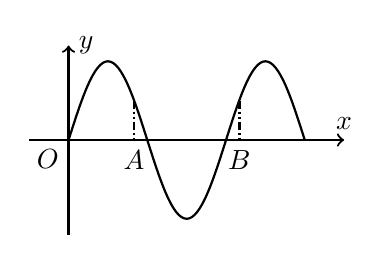
\begin{tikzpicture}
        \draw [thick,->] (-0.5,0)--(3.5,0) node [anchor=south] {$x$};
        \draw [thick,->] (0,-1.2)--(0,1.2) node [anchor=west] at (0,1.2) {$y$};
        \draw [thick] (0,0) sin (0.5,1) cos (1,0) sin (1.5,-1) cos (2,0) sin (2.5,1) cos (3,0);
        \node [anchor=north east] at (0,0) {$O$};
        \draw [thick,densely dash dot dot] (0.83,0.5)--(0.83,0) node [anchor=north] {$A$};
        \draw [thick,densely dash dot dot] (2.17,0.5)--(2.17,0) node [anchor=north] {$B$};
    \end{tikzpicture}
\vfill
\end{paracol}
\begin{solution}
    \begin{itemize}
        \item $A$点的振动动能在增大，所以$A$点在靠近平衡位置，波沿$x$轴负方向传播，B项正确
        \item 波沿$x$轴负方向传播，由图可知$B$点在远离平衡位置，其振动动能在减小，C项错误
        \item 根据机械波的特性：动能和势能同时增大或减小，能量密度随时间变化，A、D项错误
    \end{itemize}
    \sokka{B}
\end{solution}

\begin{choice}{C}[多普勒效应]
    一辆高速运动的警车发出警铃，声音频率为$f_s=1400\mathrm{Hz}$，从左向右移动，速度大小为$70\mathrm{m/s}$.一个观察者从右向左移动，速度大小为$10\mathrm{m/s}$.假设空气中没有风，空气中的声速$u=340\mathrm{m/s}$.观察者与警车相遇前后听到警铃声音的频率分别是
\begin{tasks}(4)
    \task $1711.1\mathrm{Hz},\ 1195.1\mathrm{Hz}$
    \task $1126.8\mathrm{Hz},\ 1814.8\mathrm{Hz}$
    \task $1814.8\mathrm{Hz},\ 1126.8\mathrm{Hz}$
    \task $1195.1\mathrm{Hz},\ 1711.1\mathrm{Hz}$
\end{tasks}
\end{choice}
\begin{solution}
    已知多普勒效应观察者 (Observer) 和发射源 (Source) 的频率关系为
    \[\nu=\frac{u\pm v_o}{u\mp v_s}\nu_0\]

    $v_o$为观察者速度，接近为$+$，远离为$-$；$v_s$为发射源速度，接近为$-$，远离为$+$.观察者所听频率分别为
    \[f_1=\frac{340+10}{340-70}\times 1400\mathrm{Hz}\approx 1814.8\mathrm{Hz},\ f_2=\frac{340-10}{340+70}\times 1400\mathrm{Hz}\approx 1126.8\mathrm{Hz}\]
\sokka{C}
\end{solution}

\begin{choice}{A}[迈克尔逊干涉仪]
    在迈克尔逊干涉仪的一条光路中，放入一折射率为$n$，厚度为$d$的透明薄片，放入后，这条光路的光程改变了
    \begin{tasks}(5)
        \task $2\ab(n-1)d$
        \task $2nd$
        \task $2\ab(n-1)d+\frac{\lambda}{2}$
        \task $nd$
        \task $\ab(n-1)d$
    \end{tasks}
\end{choice}
\begin{solution}*
    迈克尔逊干涉仪光路上的某点光碰到反射镜后会再次经过此处，故原来的光程为$2d$；现在加入了透明薄片，使得这里的光程为$2nd$，故光程差为$2\ab(n-1)d$.\sokka{A}
\end{solution}

\begin{paracol}{2}
    \begin{choice}{D}[双缝干涉]
        在双缝干涉实验中，用白光照射双缝隙，屏幕$E$上的$P$点明条纹外侧呈什么颜色？如果用纯绿色滤光片和纯蓝色滤光片分别盖住两缝，能否产生干涉条纹？若将缝$S_2$盖住，并在$S_1S_2$连线的垂直平分面处放一高折射率反射面$M$，如图所示.则此时P点是明纹还是暗纹？
    \begin{tasks}(2)
        \task 红色，能，明纹
        \task 蓝色，能，暗纹
        \task 蓝色，不能，明纹
        \task 红色，不能，暗纹
    \end{tasks}        
    \end{choice}
    \switchcolumn\centering
    \vfill
    \begin{tikzpicture}[decoration={markings,mark=between positions .2 and .8 step 18mm with {\arrow{stealth}}}]
        \draw [very thick] (0,1.5)--(0,-1.5);
        \draw [thick,postaction=decorate] (-1,0)--(0,0.5)--(2,0.8);
        \draw [thick] (0,0.5)--(0.8,0);
        \draw [thick,postaction=decorate] (-1,0)--(0,-0.5)--(2,0.8);
        \draw [very thick] (0,0)--(1.8,0);
        \draw [very thick] (2,1.8)--(2,-1.8);
        \fill [pattern=north west lines] (0,0) rectangle (1.8,-0.2);
        \fill [pattern=north east lines] (2,1.8) rectangle (2.2,-1.8);
        \node [anchor=east] at (-1,0) {$S$} node [anchor=south east] at (0,0.5) {$S_1$} node [anchor=north east] at (0,-0.5) {$S_2$};
        \node [anchor=north] at (0.8,-0.2) {$M$} node [anchor=west] at (2.2,0.8) {$P$} node [anchor=north] at (2.1,-1.8) {$E$};
        \node at (-1,0) {$\times$};
    \end{tikzpicture}
    \vfill
\end{paracol}
\begin{solution}
\begin{itemize}
    \item 波长越大，明纹张角越大，所以外侧呈红色
    \item 根据干涉条件「频率相等」，此时不能产生干涉条纹
    \item 光路长度不变，但平面镜使光路$\mathrm{S_1MP}$存在半波损失，两条光路的相位差变化$\pi$，所以$P$点由明纹变为暗纹.
\end{itemize}
\sokka{A}
\end{solution}

\begin{paracol}{2}
    \begin{choice}{A}[双缝干涉]
        如图所示，用波长$\lambda=600\mathrm{nm}$的单色光做杨氏双缝实验，在$P$处产生第5级明纹极大，现分别将折射率$n_1=1.75$和$n_2=1.25$的等厚薄透明玻璃片盖在两条缝上，此时$P$处变成第一级明纹极大的位置，则玻璃片厚度为
        \begin{tasks}(4)
            \task $4.8\times 10^{-4}\mathrm{cm}$
            \task $6.0\times 10^{-4}\mathrm{cm}$
            \task $7.2\times 10^{-4}\mathrm{cm}$
            \task $8.4\times 10^{-4}\mathrm{cm}$
        \end{tasks}
    \end{choice}
    \switchcolumn\centering
    \vfill
    \begin{tikzpicture}[scale=0.83]
        \draw [thick] (0,1.5)--(0,0.55);
        \draw [thick] (0,0.45)--(0,-0.45);
        \draw [thick] (0,-0.55)--(0,-1.5);
        \draw [loosely dash dot] (-0.8,0)--(5,0);
        \draw [thick] (4.5,1.8)--(4.5,-1.8);
        \fill [H6,opacity=0.4] (0,0.9) rectangle (0.2,0.1);
        \fill [H6,opacity=0.4] (0,-0.9) rectangle (0.2,-0.1);
        \draw [thick] (0,0.5)--(4.5,1.5)--(0,-0.5);
        \node [anchor=east] at (0,0.5) {$S_1$} node [anchor=east] at (0,-0.5) {$S_2$};
        \node [anchor=west] at (4.5,1.5) {$P$};
        \node [anchor=north east] at (4.5,0) {$O$};
    \end{tikzpicture}
    \vfill
\end{paracol}
\begin{solution}
    遮住前后光程差分别为
    \[\begin{cases}
        \delta_1=5\lambda=r_2-r_1\\
        \delta_2=\lambda=[r_2+(n_2-1)e]-[r_1+(n_1-1)e]
    \end{cases}\]

    联立得$5\lambda-\lambda=2400\mathrm{nm}=\ab(n_1-n_2)e$，得玻璃片厚度$e=4.8\times 10^{-4}\mathrm{cm}$.\sokka{A}
\end{solution}

\begin{paracol}{2}
    \begin{choice}{B}[劈尖干涉]
        如图所示，两个直径有微小差别的彼此平行的滚柱之间的距离为$L$，夹在两块平板透光晶体的中间，形成空气劈尖. 当单色光垂直入射时，产生等厚干涉条纹，如果两滚柱之间的距离$L$变小，或同时等比缩小两滚柱的半径，两种情况下则在$L$范围内干涉条纹的间距和级数分别会怎样？
        \begin{tasks}(2)
            \task 变大，减小；不变，变小
            \task 变小，不变；不变，变小
            \task 变小，不变；变小，变大
            \task 变小，增加；变大，变大
        \end{tasks}
    \end{choice}
    \switchcolumn\centering
    \vfill
    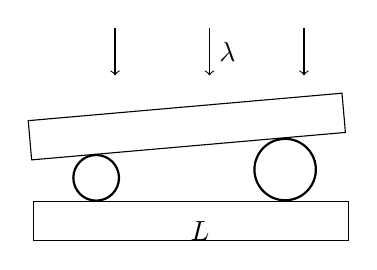
\begin{tikzpicture}
        \draw (-2,0) rectangle (2,0.5);
        \draw [rotate=5,xshift=0.78mm] (-2,1.2) rectangle (2,1.7);
        \draw [thick] (-1.2,0.8) circle (0.29);
        \draw [thick] (1.2,0.905) circle (0.39);
        \length{(-1.2,0.25)}{(1.2,0.25)}{$L$}{(0.25,0)}
        \foreach \a in {-1.2,0,1.2}
        \draw [->,xshift=\a cm] (0,2.7)--(0,2.1);
        \node [anchor=west] at (0,2.4) {$\lambda$};
    \end{tikzpicture}
    \vfill
\end{paracol}
\begin{solution}
\begin{itemize}
    \item 两滚筒间距变小相当于劈尖的顶角变大，根据条纹间距公式$\Delta x=\frac{\lambda}{2\theta}$可知条纹间隔变小；对于某条纹路，其光程差是确定的，所以数目不变.
    \item 缩小过程中空气劈形膜的顶角不变，所以条纹间隔不变，但每处的光程差减小，所以对应的条纹级数减小.
\end{itemize}
\sokka{B}
\end{solution}

\begin{choice}{C}[弗琅禾费衍射]
    在单缝夫琅和费衍射实验中，波长为$\lambda$的单色光垂直入射在宽度为$a=6\lambda$的单缝上，对应于衍射角为$30^{\circ}$的方向，单缝处波阵面可分成的半波带数目为
    \begin{tasks}(4)
        \task\color{normalcolor} 2个
        \task\color{normalcolor} 4个
        \task\color{normalcolor} 6个
        \task\color{normalcolor} 8个
    \end{tasks}
\end{choice}
\begin{solution}*
    由衍射公式$a\sin{\theta}=k\lambda$得$k=3$，可分成的半波带数目为$2k=6$.\sokka{C}
\end{solution}

\begin{paracol}{2}
    \begin{choice}{C}[弗琅禾费衍射]
    在如图所示的单缝弗琅禾费衍射装置中，将单缝宽度$a$稍稍变宽，同时使单缝沿$y$轴正方向做微小平移（透镜屏幕位置不动），则屏幕$C$上的中央衍射条纹将
    \begin{tasks}(2)
        \task\color{normalcolor} 变窄，同时向上移
        \task\color{normalcolor} 变窄，同时向下移
        \task\color{normalcolor} 变窄，不移动
        \task\color{normalcolor} 变宽，同时向上移
    \end{tasks}
    \end{choice}
    \switchcolumn\centering
    \vfill
\begin{tikzpicture}
    \filldraw [fill=gray] (0,1.5) rectangle (0.2,0.2);
    \filldraw [fill=gray] (0,-1.5) rectangle (0.2,-0.2);
    \draw [thick] (1.2,0)--(3,0);
    \draw [thick] (3,1.5)--(3,-1.5);
    \filldraw [draw=black,fill=backgroundcolor] (1.5,0) ellipse (0.1 and 1.2);
    \foreach \y in {0.8,0,-0.8}
    \draw [thick,->,yshift=\y cm] (-1,0)--(-0.5,0);
    \draw [<->] (0,-1.6)--(0,-2)--(1.6,-2);
    \node [anchor=east] at (0,-1.6) {$y$};
    \node [anchor=north east] at (0,-2) {$O$};
    \node [anchor=west] at (1.6,-2) {$x$};
    \length{(1.5,-1.4)}{(3,-1.4)}{$f$}{(0.25,0)}
    \draw [<->] (0,0.2)--(0,-0.2) node [anchor=east,midway] {$a$};
    \node [anchor=south] at (-0.5,0.8) {$\lambda$};
    \node [anchor=south] at (1.5,1.2) {$L$};
    \node [anchor=west] at (3,1.5) {$C$};
\end{tikzpicture}
    \vfill
\end{paracol}
\begin{solution}*
    光线方向不变，所以中央明纹位置不变；根据中央明纹宽度$\Delta x_0=\frac{2\lambda f}{a}$可知单缝宽度增大，中央明纹宽度将变窄.\sokka{C}
\end{solution}

